\documentclass{aastex62}

\received{September 4th, 2018}

\submitjournal{Drexel University Department of Physics}


%\shorttitle{Sample article}
%\shortauthors{Schwarz et al.}
%\newcommand{\vdag}{(v)^\dagger}
%\newcommand\aastex{AAS\TeX}
%\newcommand\latex{La\TeX}

\begin{document}

\title{WAS THE FIRST OBSERVED HYPERVELOCITY GLOBULAR CLUSTER, HVGC-1, ACCELERATED BY A SUPERMASSIVE BINARY BLACK HOLE?}

\author{Sean C. Lewis}
\affil{Drexel University Department of Physics \\
Philadelphia, Pennsylvania}



\begin{abstract}
I investigate the possibility that a supermassive binary black hole was mechanism that accelerated a hypervelocity globular cluster reported in \citet{cald14}.  Through a Monte Carlo scattering experiment, I determine the parameters necessary for a supermassive binary black hole to impart a positive energy kick to a massive particle, thereby ejecting it, or removing energy from the particle, causing it to be captured by the binary. I also determine the set of parameters that most likely would result in an extended globular cluster being accelerated to the velocity observed in \citet{cald14}. Applying thess parameters to an N-body integration using AMUSE, I find that neither a typical large cluster of  $r_{h}$ = 6 pc nor a compact cluster of $r_{h}$ = 1 pc could survive the close encounter with the black hole binary. Therefore, it is doubtful
Ultimately, I find that a cl
\end{abstract}
\section{Introduction} \label{sec:intro}
Hypervelocity objects are astrophysical objects that have been accelerated such that they are unbound from their host structure. Any such object is expected to have undergone an extreme gravitational interaction. The most common hypervelocity object directly observed are stars within the Milky Way, first predicted by \citet{hill88}.  Possible acceleration mechanisms (gravitational encounters of single stars, tidal disruptions of a stellar binary, and encounters with a binary supermassive black hole) have been explored extensively \citep{yutre03}. Now, nearly two-dozen hypervelocity stars are known. This paper will explore the posibility of another type of hypervelocity object: a globular cluster (GC). 

In 2014, a comprehensive spectroscopic survey of the massive galaxy M87 noted one particular source to have an extraordinary blueshift compared to the moderately redshifted galaxy \citep{cald14}. The source's emission spectrum was extremely blue shifted corresponding to a velocity of ~2300 km/s relative to M87. Further analysis of the object's spectrum provided modest evidence for the presence of a globular cluster, making it the first directly observed hypervelocity globular cluster, denoted as HVGC-1. In the paper reporting HVGC-1's discovery, two possible acceleration methods are proposed along with requests for further analysis through simulation. The first: the globular cluster passed between two spatially separated dark matter potentials. This possibility was addressed briefly in \citet{sam15} and will not be explored in this paper. The second possibility: HVGC-1 had a close encounter with a supermassive binary black hole (SMBBH). It has been proposed that SMBBHs are sources for some of the more extreme hypervelocity objects such as individual stars \citep{yutre03} and intracluster planetary nebulae \citep{hol05}. Although no direct observations of a binary black hole system in M87 have been made, strong evidence exists for the presence of a single supermassive black hole at the galaxy's center \citep{geb11}. In addition, it is presumed that a large galaxy like M87 has evolved through mergers (e.g., van Dokkum 2005) and, with supermassive black holes being a ubiquitous component of elliptical galaxies and spiral bulges, it is a plausible assumption that a binary black hole of comparable masses could be present in M87. 

As stated in both \citet{cald14} and \citet{sam15}, there is minimal likelihood that such an encounter could produce an intact globular cluster. It may be the case that, in order to receive a significant velocity kick, the cluster must pass within 10 parsecs of the BBH. Indeed, Caldwell presents scenarios in which a $2\times10^6M_{sun}$ cluster passes 2--3 pc from the supermassive black hole, an interaction in which the tidal radius on the globular cluster would be 0.3--0.4 pc. Undoubtedly, for a cluster of presumed radius ~6--10 pc, this would be a devastating event, potentially resulting in only the core of the cluster surviving. However, a simple keplerian calculation reveals the time spent in the vicinity of the SMBBH is small, on the order of 5000 years. So, the cluster will experience the extreme tidal forces in the form of nearly a delta function. In addition, if outer stars are being stripped from the cluster, the change in mass may result in a higher exit velocity, making the achievability of ``hypervelocity" more reasonable. It is the goal of this paper and analysis to determine the fate of such a globular cluster. 

\section{Creating a simple gravity slingshot}
\subsection{Overview}
The Astrophysical Multipurpose Software Environment \citep{zwart18} is used to accurately model and analyze the behavior of a globular cluster and its constituent stars during its close pass with a SMBBH. AMUSE uses an integrator to evolve a gravitational system while also allowing the user to pause the integration and record data such as particle mass, position, velocity, and energy. I chose to use the N-body integrator ph4. I begin by finding an idealized point-mass (test particle) trajectory, the particle paths that result in the largest velocity kick, in a Monte Carlo scattering simulation. The set of varied parameters will be discussed throughout Section 2 and subsection 2.6. In each iteration of the simulation, the test particle will pass the black hole binary in a prograde planar orbit. Such an orbit will maximize the time the test particle will spend in a close proximity to either binary component of the black hole system, thereby maximizing the energy transferred. I end by using the ideal set of parameters, maximizing the ejection velocity and minimizing external tidal accelerations, to observe and analyze the effects on the structure of a cluster containing {\raise.17ex\hbox{$\scriptstyle\mathtt{\sim}$}}1000 point masses. 

\subsection{Initial Conditions}
I began my simulation by generating and evolving a simple 3-body interaction. Two of the bodies represented the supermassive black holes: each were given an appropriate mass and orbit parameters based on user-defined total mass, mass ratio, and constant separation distance. The relative motion of the two SMBBH components was assumed to be circular. The initial position and velocity components of the black hole particles were calculated using basic orbital mechanics and trigonometry. I will refer to the ``phase" of the black holes throughout this paper. If both black holes were placed along the x-axis at the beginning of integration, the black holes are said to have a phase of 0 radians. A phase of $\pi/2$ radians corresponds to the black holes lying on the y-axis. The code also places a globular cluster particle at a distance of {\raise.17ex\hbox{$\scriptstyle\mathtt{\sim}$}}120 pc away from the black hole binary in the same plane as the binary orbits. The distance is an estimate because, in addition to being initially displaced from the SMBBH by set 100 pc along the y-axis, the GC is offset along the x-axis by the impact parameter of the interaction. The impact parameter, or the GC's distance of closest approach, will be used as a primary Monte Carlo scattering parameter. The impact parameter is calculated by examining the conservation of energy and angular momentum of a test particle as it travels from ``infinity" to its closest approach to the black holes. Specifically, this is a 2-body approximation since, for any large distance from the point of closest approach, the black hole binary appears as a single point mass:
\begin{equation}
\frac{1}{2}v_{\infty}^2 = \frac{1}{2}v_{c}^2 - \frac{GM_{BH}}{r_{c}}
\end{equation}
\begin{equation}
L = v_{\infty}b = v_{c}r_{c}
\end{equation}
\begin{equation}
b = r_{c}\sqrt{1+\frac{GM_{BH}}{r_{c}v_{\infty}^2}}
\end{equation}
Where $v_{\infty}$ is the GC initial velocity far from the black hole binary, $v_{c}$ is the GC velocity at closest approach, G is the gravitational constant, $M_{BH}$ is the total mass of the black hole binary, $r_{c}$ is the GC's closest approach to the BBH center of mass, and b is the impact parameter.  The quantities $v_{\infty}$ and $M_{BH}$ were held fixed at 500 km/s and $7 \times 10^9 M_{\odot}$ respectively. So, by asserting a distance of closest approach, AMUSE will generate a simulation in which the GC falls towards the SMBBH, undergoes a prograde planar interaction, and then have the GC's ejection velocity recorded once it reaches 120 pc away from the BBH. 

\subsection{Mirroring HVGC-1}
There is limited information on the distance of HVGC-1 from the center of M87. Any assertion as to its value is constrained by two things. First, the vast majority of HVGC-1's velocity must be in the radial direction, towards Earth, rather than the tangential direction. If this were not the case, the object's total  velocity would be even more extreme, an unlikely occurrence for an object whose velocity is already a 7$\sigma$ outlier. Secondly, HVGC-1's tangential velocity must be large enough such that the object can achieve a tangential distance of 85 kpc with respect to M87 within a short enough time that the object does not travel significantly far away from M87 in the radial direction. With these two considerations, I very roughly estimate HVGC-1 to be between 1 Mpc and 5 Mpc from M87. This, in tandem with the estimation of the potential well of M87, an object's exit velocity (recorded in my simulation at 120 pc away from the SMBBH) must be on the order of 3000 km/s for it to have an observed velocity of 2300 km/s at the estimated distance of HVGC-1 (see Figure \ref{fig1}). A distance of a few megaparsecs corresponds to a total travel time of about 1 gigayear. I explore parameters of the binary black hole system that permit a significant exit velocity and examine specific scenarios that might allow a star cluster to survive the interaction and exhibit velocities similar to those observed in \citet{cald14}.

By examining the galactic potential of M87, a rough estimate can be made for the necessary ejection velocity of an object recorded at 120 pc from the galactic center in order to possess a velocity of 2300 km/s at a significantly further radial distance. Assuming a power-law density model where the mass density behaves as $\rho(r) = \rho_{o}(r_{o}/r)^\alpha$ and the mass within radius r is $M(r) = (4\pi G\rho_{o}r_{o}^\alpha r^{3-\alpha})/(3-\alpha)$, the potential difference at two different radii can be calculated:
\begin{equation}
\Delta\Phi = \Phi(r) - \Phi(r_{o}) = G\int_{r_{o}}^{r} \! \frac{M(r')}{r'^2} \, \mathrm{d}r' = \frac{4\pi G\rho_{o}r_{o}^\alpha }{3-\alpha} r^{3-\alpha}\int_{r_{o}}^{r} \! r'^{1-\alpha} \, \mathrm{d}r'
\end{equation}
 $\alpha$ would be equal to 2 under the assumption the mass density of the galaxy is proportional to $r^{-2}$. So,
\begin{equation}
 %= \frac{v_{c}^{2}(r_{o}) - v_{c}^{2}(r)}{\alpha - 2} for \alpha \neq 2
 \Delta\Phi= v_{c}^{2}\ln(r/r_{o})
\end{equation}
Where $v_{c}$ is the circular velocity, which I take here to be equivalent to the velocity dispersion of M87: 500 km/s, $r$ is the distance from M87 at which HVGC-1 is thought to be, $\gg$85 kpc, and $r_{o}$ is the distance from the galactic center at which my simulation ends and records an ejection velocity, 120 pc. 

This is acceptable for this order-of-magnitude estimation, although it has been noted that more complicated multi-moment potentials may be present in and around M87 \citep{mur14}. In addition, as stated before, the dark matter potential of M87 is a more significant potential. I have decided a model of the dark matter halo potential of M87 will produce a more accurate understanding of an object's velocity as it leaves the galaxy \citep{zhu14}. 

Using data from long-orbit globular clusters around M87, \citet{zhu14} developed a dark matter potential model to aid in the analysis of M87 galactic dynamics. They find:
\begin{equation}
\Delta\Phi = \frac{V_{s}}{2}(ln(R_{s}^2 + r^2) - ln(R_{s}^2 + r_{o}))
\end{equation}

By setting the change in kinetic energy equal to equation 6, we find the velocity at some distance, r, from the center of M87 to be:
\begin{equation}
v_{f} = \sqrt{v_{i}^2 + V_{s}^{2}[\ln(R_{s}^2 + r^2) - \ln(R_{s}^2 + r_{o}^2)]}
\end{equation}

\begin{figure}
\figurenum{1}
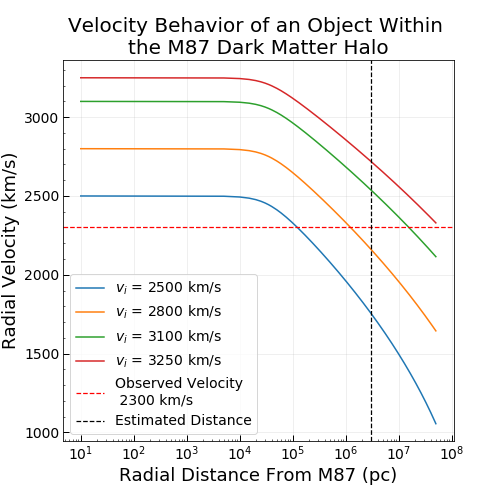
\includegraphics[width=9cm,height=9cm]{./Images/velocity_behavior.png}
\centering
\caption{text\label{fig1}}
\end{figure}

\begin{figure}
\figurenum{2}
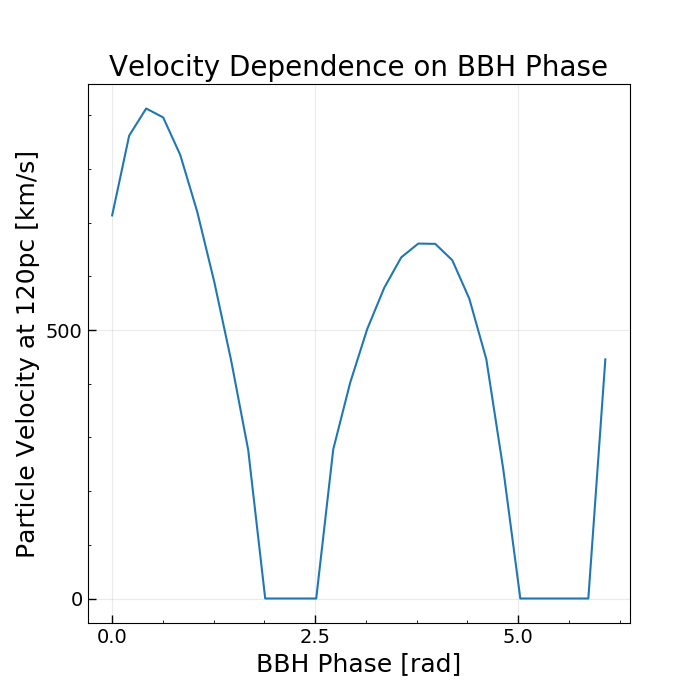
\includegraphics[width=9cm,height=9cm]{./Images/phase_loop.png}
\centering
\caption{text\label{fig2}}
\end{figure}

 It should be noted, although I am taking the galactic potential into consideration to gain insight into the ejection velocity and total integration time, the potential is not taken to account in analyses of the N-body interaction since the question of cluster survivability depends little on the presence of a galactic potential. 
\subsection{Cluster Exit Velocity and BH Phase Dependence}
The cluster's exit velocity depends heavily on the phase of the black holes during its closest approach to the binary. In order to determine the ideal phase of the BH's during the interaction, the simulation was repeated while varying the initial locations of the black holes in their orbit. This is equivalent to varying the BH phase during closest approach. The result is: a BH phase-dependent exit velocity that clearly shows two peaks corresponding to the cluster arriving at the SMBBH while the outer and inner BH are in phase with it, see Figure \ref{fig2}.

Interestingly, some BH phases result in the test particle becoming captured by the binary black hole system. An easy check to confirm a gravity capture is taking place (as opposed to some odd unintended consequence within the AMUSE code) is to investigate the test particle's energy during the interaction. It would be expected that the particle's total energy relative to the center of mass of the system is a conserved quantity, that is, until a close pass with the SMBBH whereafter the particle's energy will be lower. Indeed, this is what is observed, see \ref{fig3}. For comparison, an interaction that results in the ejection of the GC will have the GC's relative energy also remain constant as it infalls towards the SMBBH, then have a positive shift after the interaction, see Figure \ref{fig3}. Interactions that result in a captured GC test particle were discarded and not considered further as this investigation focuses only on the possibility of a GC being ejected at greater than 1000 km/s, but such interactions may be useful for further simulations regarding stellar or more complex structure capture by binary black holes.
\begin{figure}
\figurenum{3}
\plottwo{./Images/bound_track_new.png}{./Images/bound_energy.png}
\caption{Left: The globular cluster (red path) begins its path at the bottom right at (38 pc, -100 pc) and begins infalling towards the black hole binary (black path: more massive BH, blue path: less massive BH. Notice how the GC appears to be tracing a path that is beginning to turn back around towards the SMBBH. Right: The relative energy, in Joules, of the globular cluster during throughout its journey towards, around, and away from the SMBBH. The oscillation and large spike are due to the gravitational potential close to the SMBBH becomes more significantly more complex than the assumed point mass viewed from infinity. Here, the GC begins at -3.15E48 J of relative energy and ends with -4.42E48 J, a 40.3\% decrease in energy relative to the center of mass of the system.\label{fig3}}
\end{figure}
\begin{figure}
\figurenum{4}
\plottwo{./Images/ejection_track.png}{./Images/unbound_energy.png}
\caption{Left: All initial conditions are equal to those in Figure 1 except for the location of the black holes in their orbit during the GC's closest pass. Notice, the GC (red line) makes a much more direct path away from the SMBBH than in Figure 1. Right: After its interaction with the SMBBH, the GC has gained relative energy and has been ejected from the system. Here, the GC begins with -3.15E48 J of energy (the same as in Figure 1) and ends with +1.94E48 J, a 161.6\% increase in energy.\label{fig4}}
\end{figure}
\subsection{Operational Parameters}
The parameters of the prograde planar Monte Carlo scattering study were the BH mass ratio, the separation of the BHs, the GC's closest approach, and BH phase. These values were varied to explore the parameter space in an attempt to determine the combination that resulted in the highest GC exit velocity and smallest tidal perturbation: $\gamma = {a_{t}}/{a_i}$ where $a_{t}$ is the tidal acceleration of the GC due to the presence of the external BH gravity well and $a_{i}$ is the internal acceleration of the GC. A small tidal perturbation implies a higher likelihood of a significant fraction of the star cluster surviving the interaction. To explore a large range of parameter space, the following were chosen: BH mass ratio [0.01, 0.05, 0.1, 0.25], BH semimajor axis (pc) [1.7, 3.0, 5.0], GC closest approach (number of times greater than the BH Axis) [1.5, 2, 2.5]. With each combination of parameters, the interaction was repeated with initial BH phases varying by steps in $\pi/15$ so that the most optimum orientation of the BHs can be isolated and investigated further. 

\subsection{Optimum Interaction}
In total, 1,080 simulations were run and only 147 resulted in an GC test-particle exit velocity exceeding 1000 km/s, satisfying the ``hypervelocity" condition. Each interaction also recorded the tidal perturbation experienced. Of the 147 trials, I chose three that were of particular interest, see Table \ref{results}. The first interaction listed has the highest velocity to tidal perturbation ratio out of all of the interactions, meaning the largest exit velocity and a small tidal perturbation compared to other interactions with ejections of comparable velocities. The second interaction listed has the highest velocity to perturbation ratio for an event resulting in a velocity $>$2000 km/s. The third has the highest ratio for an interaction with a $>$3000 km/s exit velocity. Notice, all three interaction involve a BBH mass ratio of 0.25, as did the majority of the 147 hypervelocity interactions (63$\%$). In fact, there were zero interaction that resulted in a hypervelocity exit by the test particle for a BH mass ratio of 0.01. A higher mass ratio allows the GC to receive a substantial velocity kick while remaining further away from the black hole binary, resulting in a lower tidal perturbation, although, to describe the tidal perturbation as ``low" would be to misrepresent the nature of the encounter. Even in the ideal survival scenario (the first interaction in Table \ref{results}), the tides experienced by the GC due to the presence of BH masses $M_{1}$ and $M_{2}$ reach a respective maximum at 650 and 693 times the internal acceleration of the star cluster. This highlights the extraordinary nature of the encounter, and implies that the cluster will almost certainly be torn apart unless the tidal ratio remains high for only a brief time period. 

The encounter that is most capable of mirroring HVGC-1's current behavior is the third entry in Table \ref{results}, where the star cluster briefly experiences a tidal acceleration 67,621 times its internal acceleration. These two interactions were chosen for further analysis as the first satisfies the condition of the production of a hypervelocity object, and the second satisfies initial velocity conditions necessary for HVGC-1's extraordinary behavior. The ``ideal-ness" of these three encounters can be refined in the future. However, in my opinion, doing so would reduce an already unlikely scenario down to a near impossible set of perfect circumstances. For the purposes of determining the survivability of a star cluster, these ``ball-park" parameters will suffice. 

\begin{table}
\centering
\caption{Interactions of interest. Columns from left to right: Exit velocity of the GC 120 pc away from the BBH, mass ratio of the black holes, BH separation distance, Minimum distance from the binary center of mass achieved by the GC, Initial BH phase, Maximum tidal perturbation experienced by the GC due to $M_{1}$ (more massive component), Maximum tidal perturbation due to $M_{2}$. \label{results}}

\begin{tabular}{ccccccc}
\hline \hline
Velocity (km/s) & $M_{2}/M_{1}$ & BH Axis (pc) & Min Dist. (pc) & BH $\Phi$ (rad) & $\gamma_{1}$ & $\gamma_{2}$  \\
1124 & 0.25 & 5.0 & 8.5 & 5.24 & 650 & 692 \\
2336 & 0.25 & 3.0 & 4.5 & 4.61 & 4771 & 7768 \\
3436 & 0.25 & 1.7 & 2.5 & 1.47 & 28584 & 67621 \\
\end{tabular}
\end{table}

%\subsection{Comparison to HVGC-1}
%The object highlighted in \citet{cald14} was determined to be traveling at {\raise.17ex\hbox{$\scriptstyle\mathtt{\sim}$}}2300 km/s outwards from M87 at a distance of 84 kpc


\section{A Close Pass of a GC with a SMBBH}
\subsection{Initializing the Simulation}
To determine a cluster's survivability, the test particle must be extended to a self-gravitating cluster. AMUSE is perfect for such a simulation and analysis, with built in N-body integrators and cluster generators. Specifically, I use a \citet{plum11} model globular cluster consisting of 1000 particles each with a mass of $10^4 M_{\odot}$, resulting in a total cluster mass of $10^7 M_{\odot}$. The choice of 1000 particles was made to ease the processing needs of the simulation. Increasingly accurate simulations are possible at the expense of computational time. For the purposes of this analysis, this approximation was considered sufficient. Creation of the simulation simply required the insertion of said cluster particle set into the perviously used test particle code, reasserting chosen ideal parameters from Table \ref{results}, and integrating for a user-specified amount of time. The final parameter that can still be varied is the half-mass radius, $r_{h}$, of which I have chosen to investigate  $r_{h}$ = 6 pc and 1 pc. A value of 6 pc corresponds to the estimated current radius of the cluster, and 1 pc is an optimized scenario of a hyper-compact galaxy core. Presumably, a 1 parsec  $r_{h}$ would more likely result in one or more particle clusters surviving the interaction. In addition, I introduced a smoothing parameter of 0.05 times the given radius of the cluster (0.05 pc and 0.3 pc respectively). Any particles encountering each other at a smaller distance will have their interaction smoothed, easing computational requirements by eliminating hard interactions. 
\subsection{Results of the Encounter}
Using the parameters for the test case that resulted in the highest final velocity, the globular cluster and its resulting destruction was followed for 200 kyr, 1 Myr, 2 Myr, 20 Myr, and 2 Gyr which were plotted for visual inspection and further analysis. The 2 Gyr aftermath of a $r_{h}$ = 1 pc, and 6 pc GC SMBBH encounters can be seen in Figure \ref{fig5}. 

\begin{figure}
\figurenum{5}
\plottwo{./Images/1pc2Gyr_scatter.png}{./Images/6pc2Gyr_scatter.png}
\centering
\caption{Top-down view of 2 billion years after a $r_{h}$ = 1 pc (left), and 6 pc (right) globular cluster encountered a SMBBH. Each point represents $10^3 M_{\odot}$. The center of mass for the entire cluster is marked in red. The radius of M87 (the host galaxy from which these clusters would have originated from) is on the order of 50 kpc. The "structure" in these images is extraordinarily diffuse, and would be extending to the edge of the virgo galaxy cluster.\label{fig5}}
\end{figure}

Surprisingly, the hyper-compact cluster appears, at least upon visual inspection, to be more dispersed or disrupted compared to the 6 pc cluster. This is confirmed by the 6 pc cluster's center of mass being more distant from the place of interaction, (0,0). However, further analysis of the center of mass location of a tidally disrupted star cluster is fruitless unless the constituent particles are given enough time to relax and possibly coalesce into smaller clusters. In order to determine whether any fragment of the original cluster will recombine and form another smaller cluster, I employed two simple analysis methods, first, I calculated how the number of cluster particles that were bound to the BBH in each integration step mentioned previously. It is expected that all cluster particles begin as bound to the SMBBH as seen in the total relative energy plots of my scattering analysis, Figures 2 and 3. After 200 kyr, the SMBBH will have imparted enough energy to some of the particles to eject them from the system. If any particles are still bound to the SMBBH, they will eventually become unbound as they continue to orbit the binary, undergoing a type of random-walk as their relative energy increases or decreases with each close encounter with the binary. Eventually, none of the cluster particles are expected to be bound to the SMBBH. Indeed, this is what is seen in Figure 5; with only 5 data points, a higher resolution analysis is certainly possible, but ultimately the system's behavior is as expected.
\begin{figure}
\figurenum{6}
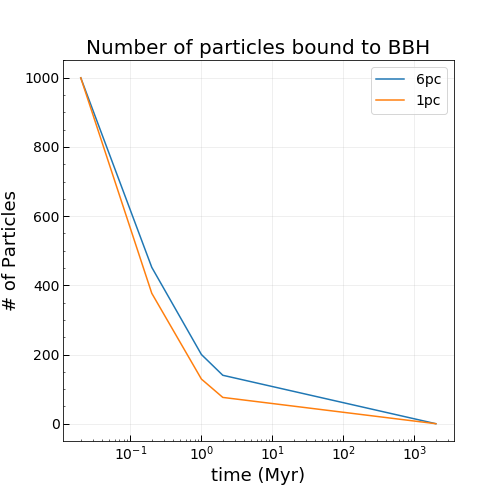
\includegraphics[width=9cm,height=9cm]{./Images/bound_particle_number.png}
\centering
\caption{The evolution of number of bound particles originally constituents of the two analyzed clusters. As expected, each cluster seems to have been heavily disrupted very soon after a close pass to a SMBBH, with nearly a 50-50 split between particles ejected from the system and particles remaining bound. And, predictably, more particles become unbound from the SMBBH as repeated close encounters eventually kick each particle out.\label{fig6}}
\end{figure}

The second, more rigorous analysis was the use of a cluster-identifying software built into AMUSE known as the HopInterface \citep{eisen98} to determine the point of greatest density within any individualized groups within the 2 Gyr old particle set. HOP identifies a collection of particles as a "group" based on the mass density of the space occupied by a particle. If a region of particles satisfy the peak density threshold as well as an appropriate number of neighbors to the point of greatest density, HOP defines the surrounding particles as a group. For the purposes of this analysis, I maintained the threshold parameters at their default values, meant specifically for cluster group identification. The most important parameter would be the number of neighboring particles that would constitute a group, 64 in this case. A 64 particle group would represent a $6.4 * 10^5 M_{\odot}$ cluster, potentially a small globular cluster. The grouping results can be seen plotted in Figure 6. Interestingly, given the same operational parameters, the HopInterface identified 3 separate groups within the disrupted 6 parsec radius cluster and was unable to identify any subgroups of the disrupted 1 parsec cluster. This is consistent with a visual inspection of the scatter plots: the 1pc cluster does appear to have less well-defined structure. However, in both cases, and in all subgroups, the point of maximum density were all less than $0.3 \frac{M_{\odot}}{kpc^3}$ representing a very diffuse system which could not qualify as a globular cluster which can have as many as $100$ to $1000 \frac{\text{stars}}{pc^3}$ in their cores. It can then be said with confidence, that both cluster's close encounters with a SMBBH did not produce a hypervelocity globular cluster, or a globular cluster of any kind. However, the BBH did manage to eject all particles from their previously bound states implying the production of many individual hypervelocity stars.

\begin{figure}
\figurenum{7}
\plottwo{./Images/groups_1pc2Gyr.png}{./Images/groups_6pc2Gyr.png}
\centering
\caption{Plot Legends: List each subgroup identified within the disrupted particles and their corresponding fraction of total mass. Each cluster has a total mass of $10^7 M_{\odot}$. The black x represents the point of greatest density within each subgroup. Left plot density points: $0.066 \frac{M_{\odot}}{kpc^3}$. Right plot density points: $0.289 \frac{M_{\odot}}{kpc^3}$, $0.004 \frac{M_{\odot}}{kpc^3}$, and $0.054 \frac{M_{\odot}}{kpc^3}$ for the green, orange, and purple groups respectively.\label{fig7}}
\end{figure}

\section{Conclusion}
I have studied the close encounter of a $r_{h} = 6$ parsec and $r_{h} = 1$ parsec $10^7$ $M_{\odot}$ globular cluster with a $7*10^9 M_{\odot}$ 1:4 mass ratio binary black hole system to investigate the possibility of a cluster-like structure surviving the encounter. I attempt to verify the possibility that such an encounter could produce an object similar to the one observed in \citet{cald14}, denoted as HVGC-1. 

Through a simple three-body scattering experiment, I was able to constrain a set of parameters to produce an accelerated test particle that mirrored the extraordinary velocity behavior of HVGC-1. In the process, I found that the orientation of the binary components of the supermassive black hole determines whether the test particle is given an energy kick, or is dragged down into a more deeply bound orbit. This may be an interesting interaction that could be further explored to constrain the ejection rate of stars orbiting a binary black hole. Once an optimum set of parameters was determined, it was used as initial conditions for an N-body simulation: expanding the $10^7$ $M_{\odot}$ test particle into a Plummer model based cluster consisting of 1000 particles. Data was returned from the N-body simulation at 200 kyr, 1 Myr, 2 Myr, and 2 Gyr. Further analysis revealed the number of cluster particles bound to the supermassive binary black hole decreases as a function of time as expected. The 2 Gyr time-step was investigated further using the HopInterface to reveal any defined subgroups within the disturbed cluster as well as the groups' density peaks. Hop identified 3 subgroups in the $r_{h} = 6$ pc and 0 subgroups in the $r_{h} = 1$ pc cluster. In all cases, the density peak remained below $0.3$ solar masses per cubic kiloparsec, implying that no tightly bound structure survived the interaction. 

Ultimately I determined that a close encounter with a supermassive binary black hole that produced a test particle with characteristics most like the observed HVGC-1 completely destroys a generically size and compact globular cluster. Therefore, it is likely that HVGC-1 was not accelerated by a close encounter with a SMBBH. It may be possible to create a hypervelocity cluster with a velocity significantly less than that observed in HVGC-1, and the necessary BH parameters for such an object have already been explored in my test particle scattering experiment. Further investigation into this prospect would aid in answering the question: can a SMBBH produce a hypervelocity globular cluster under any circumstances? A more rigorous analytical approach and refined simulation techniques may be necessary to fully and accurately explore the large and computationally demanding parameter space.

\begin{thebibliography}{}
\bibitem[Caldwell et al.(2014)]{cald14} 
Caldwell, N., Strader, J., Romanowsky, A. J., et al. 2014, \apjl, 787, L11
\bibitem[Eisenstein, DJ., Hut, P.(1998)]{eisen98}
Eisenstein, DJ., Hut, P., 1998, HOP: A new group-finding algorithm for N-body simulations, \apj, 498
\bibitem[Gebhardt et al.(2011)]{geb11}
Gebhardt, K., Adams, J., Richstone, D., et al. 2011, \apj, 729, 13
\bibitem[Hill(1988)]{hill88}
Hill, J. G., 1988, Nature, 331
\bibitem[Holley-Bockelmann et al.(2005)]{hol05}
Holley-Bockelmann et al. 2005, \apjl
\bibitem[Murphy, J., Gebhardt, K., Craidt, M.(2014)]{mur14}
Murphy, J., Gebhardt, K., Craidt, M. 2014, \apj
\bibitem[Plummer(1911)]{plum11}
Plumer, H.C. 1911. On the problem of distribution in globular star clusters. MNRAS, 71(Mar.), 460-470.
\bibitem[Sesana et al.(2008)]{ses08}
Sesana, A., Haardt, F., Madau, P. 2008, \apj, 686
\bibitem[Samsing(2015)]{sam15}
Samsing, J. 2015, \apj, 799, 11
\bibitem[Yu \& Tremaine(2003)]{yutre03}
Yu \& Tremaine. 2003, \apj, 599
\bibitem[Zhu et al.(2014)]{zhu14}
Zhu, L., Long R. J., Mao, Shude, et al. 2014 \apj
\bibitem[Zwart \& McMillan(2018)]{zwart18}
Zwart, S. P., McMillan, S. (2018). \textit{Astrophysical Recipes The Art of AMUSE}. Institute of Physics Publishing
\end{thebibliography}
\end{document}
